\subsection{Peripheral Component Interconnect Express (\gls{pcie})}
The PCI architecture has proven to be successful beyond even the most optimistic expectations. Today nearly every new computer platform comes outfitted with multiple PCI slots. In addition to the unprecedented number of PCI slots being shipped, there are also hundreds of PCI adapter cards that are available to satisfy virtually every conceivable application. This enormous momentum is difficult to ignore.

Today there is also a need for a new, higher-performance I/O interface to support emerging, ultrahigh-bandwidth technologies such as 10 Gigabit Ethernet, 10 Gigabit FibreChannel, 4X and 12X InfiniBand, and others. A standard that can meet these performance objectives, while maintaining backward compatibility to previous generations of PCI would undoubtedly provide the ideal solution.

To meet these objectives, the PCI-X 2.0 standard has been developed. PCI-X 2.0 has the performance to feed the most bandwidth-hungry applications while at the same time maintaining complete hardware and software backward compatibility to previous generations of PCI and PCI-X. The PCI-X 2.0 standard introduces two new speed grades: PCI-X 266 and PCI-X 533. These speed grades offer bandwidths that are two times and four times that of PCI-X 133 -- ultimately providing bandwidths that are more than 32 times faster than the original version of PCI that was introduced eight years ago. It achieves the additional performance via time-proven DDR (Double Data Rate) and QDR (Quad Data Rate) techniques that transmit data at either 2-times or 4-times the base clock frequency. Because PCI-X 2.0 preserves so many elements from previous generations of PCI it is the beneficiary of a tremendous amount of prior development work. The operating systems, connector, device drivers, form factor, protocols, BIOS, electrical signaling, BFM (bus functional model), and other original PCI elements, are all heavily leveraged in the PCI-X 2.0 specification.

In fact, many of these elements remain identical in PCI-X 2.0. These similarities make implementation easy because these elements have already been designed and engineers are already familiar with them. As a result, the time-to-market is short, and risk is dramatically reduced.

The market migration to PCI-X 2.0 will also be easy because there are so many previous-generation PCI adapter cards already on the market. There are already hundreds of PCI adapter cards that are available today that can be utilized by every PCI-X 266 and PCI-X 533 slot. In addition, new PCI-X 266 and PCI-X 533 adapter cards have ready homes in any of the millions of PCI and PCI-X slots in existing systems. Because of these factors, PCI-X 2.0 provides the ideal next-generation, local I/O solution for high-bandwidth applications. It offers the performance needed for today’s and tomorrow’s applications in an easy-to-adopt, backward-compatible standard.

\subsubsection{Functional Description}
PCI BIOS functions provide a software interface to the hardware used to implement a PCI based system. Its primary usage is for generating operations in PCI specific address spaces (configuration space and Special Cycles).
PCI BIOS functions are specified to operate in the following modes of the X86 architecture. The modes are: real-mode, 16:16 protected mode (also known as 286 protected mode), 16:32 protected mode (introduced with the 386), and 0:32 protected mode (also known as “flat” mode, wherein all segments start at linear address 0 and span the entire 4-GB address space).

Access to the PCI BIOS functions for 16-bit callers is provided through Interrupt 1Ah. 32-bit (i.e., protected mode) access is provided by calling through a 32-bit protected mode entry point. The PCI BIOS function code is B1h. Specific BIOS functions are invoked using a sub-function code. A user simply sets the host processors registers for the function and sub-function desired and calls the PCI BIOS software. Status is returned using the CARRY FLAG ([CF]) and registers specific to the function invoked.

\subsubsection{UEFI PCI Services}
UEFI stands for Unified Extensible Firmware Interface. The UEFI Specification, Version 2.3 or later describes an interface between the operating system and the platform firmware. The interface is in the form of data tables that contain platform-related information and boot and run-time services calls that are available to the operating system and its loader. Together, these provide a standard environment for booting an operating system.

The following sections provide an overview of the EFI Services relevant to PCI (including Conventional PCI, PCI-X, and PCI Express). For details, refer to the UEFI Specification. UEFI is processor-agnostic.


\subsubsection{UEFI Driver Model}
The UEFI Driver Model is designed to support the execution of drivers that run in the pre-boot environment present on systems that implement the UEFI firmware. These drivers may manage and control hardware buses and devices on the platform, or they may provide some software derived platform specific services.

The UEFI Driver Model is designed to extend the UEFI Specification in a way that supports device drivers and bus drivers. It contains information required by UEFI driver writers to design and implement any combination of bus drivers and device drivers that a platform may need to boot an UEFI-compliant operating system.

Applying the UEFI Driver Model to PCI, the UEFI Specification defines the PCI Root Bridge Protocol and the PCI Driver Model and describes how to write PCI bus drivers and PCI devices drivers in the UEFI environment. For details, refer to the UEFI Specification.

\begin{itemize}
	\item \textbf{PCI Root Bridge Protocol} - A PCI Root Bridge is represented in UEFI as a device handle that contains a Device Path Protocol instance and a PCI Root Bridge Protocol instance. PCI Root Bridge Protocol provides an I/O abstraction for a PCI Root Bridge that the host bus can perform. This protocol is used by a PCI Bus Driver to perform PCI Memory, PCI I/O, and PCI Configuration cycles on a PCI Bus. It also provides services to perform different types of bus mastering DMA on a PCI bus. PCI Root Bridge Protocol abstracts device specific code from the system memory map. This allows system designers to make changes to the system memory map without impacting platform independent code that is consuming basic system resources. An example of such system memory map changes is a system that provides non-identity memory mapped I/O (MMIO) mapping between the host processor view and the PCI device view.
	\item \textbf{PCI Driver Model} - The PCI Driver Model is designed to extend the UEFI Driver Model in a way that supports PCI Bus Drivers and PCI Device Drivers. This applies to Conventional PCI, PCI-X, and PCI Express. PCI Bus Drivers manage PCI buses present in a system. The PCI Bus Driver creates child device handles that must contain a Device Path Protocol instance and a PCI I/O Protocol instance. The PCI I/O Protocol is used by the PCI Device Driver to access memory and I/O on a PCI controller. PCI Device Drivers manage PCI controllers present on PCI buses. The PCI Device Drivers produce an I/O abstraction that may be used to boot an UEFI compliant operating system.
\end{itemize}

\subsubsection{BUS Performances and Number of Slots Compared}
The various architectures defined by the PCISIG. The table shows the evolution of bus frequencies and bandwidths., as it obvious, increasing bus frequency compromises the number of electrical loads or number of connectors allowable on a bus at that frequencies. At some point for a given bus architecture there is an upper limit beyond which one cannot further increase the bus frequency, hence requiring the definition of a new bus architecture.

\begin{figure}[!htbp]
	\centering
	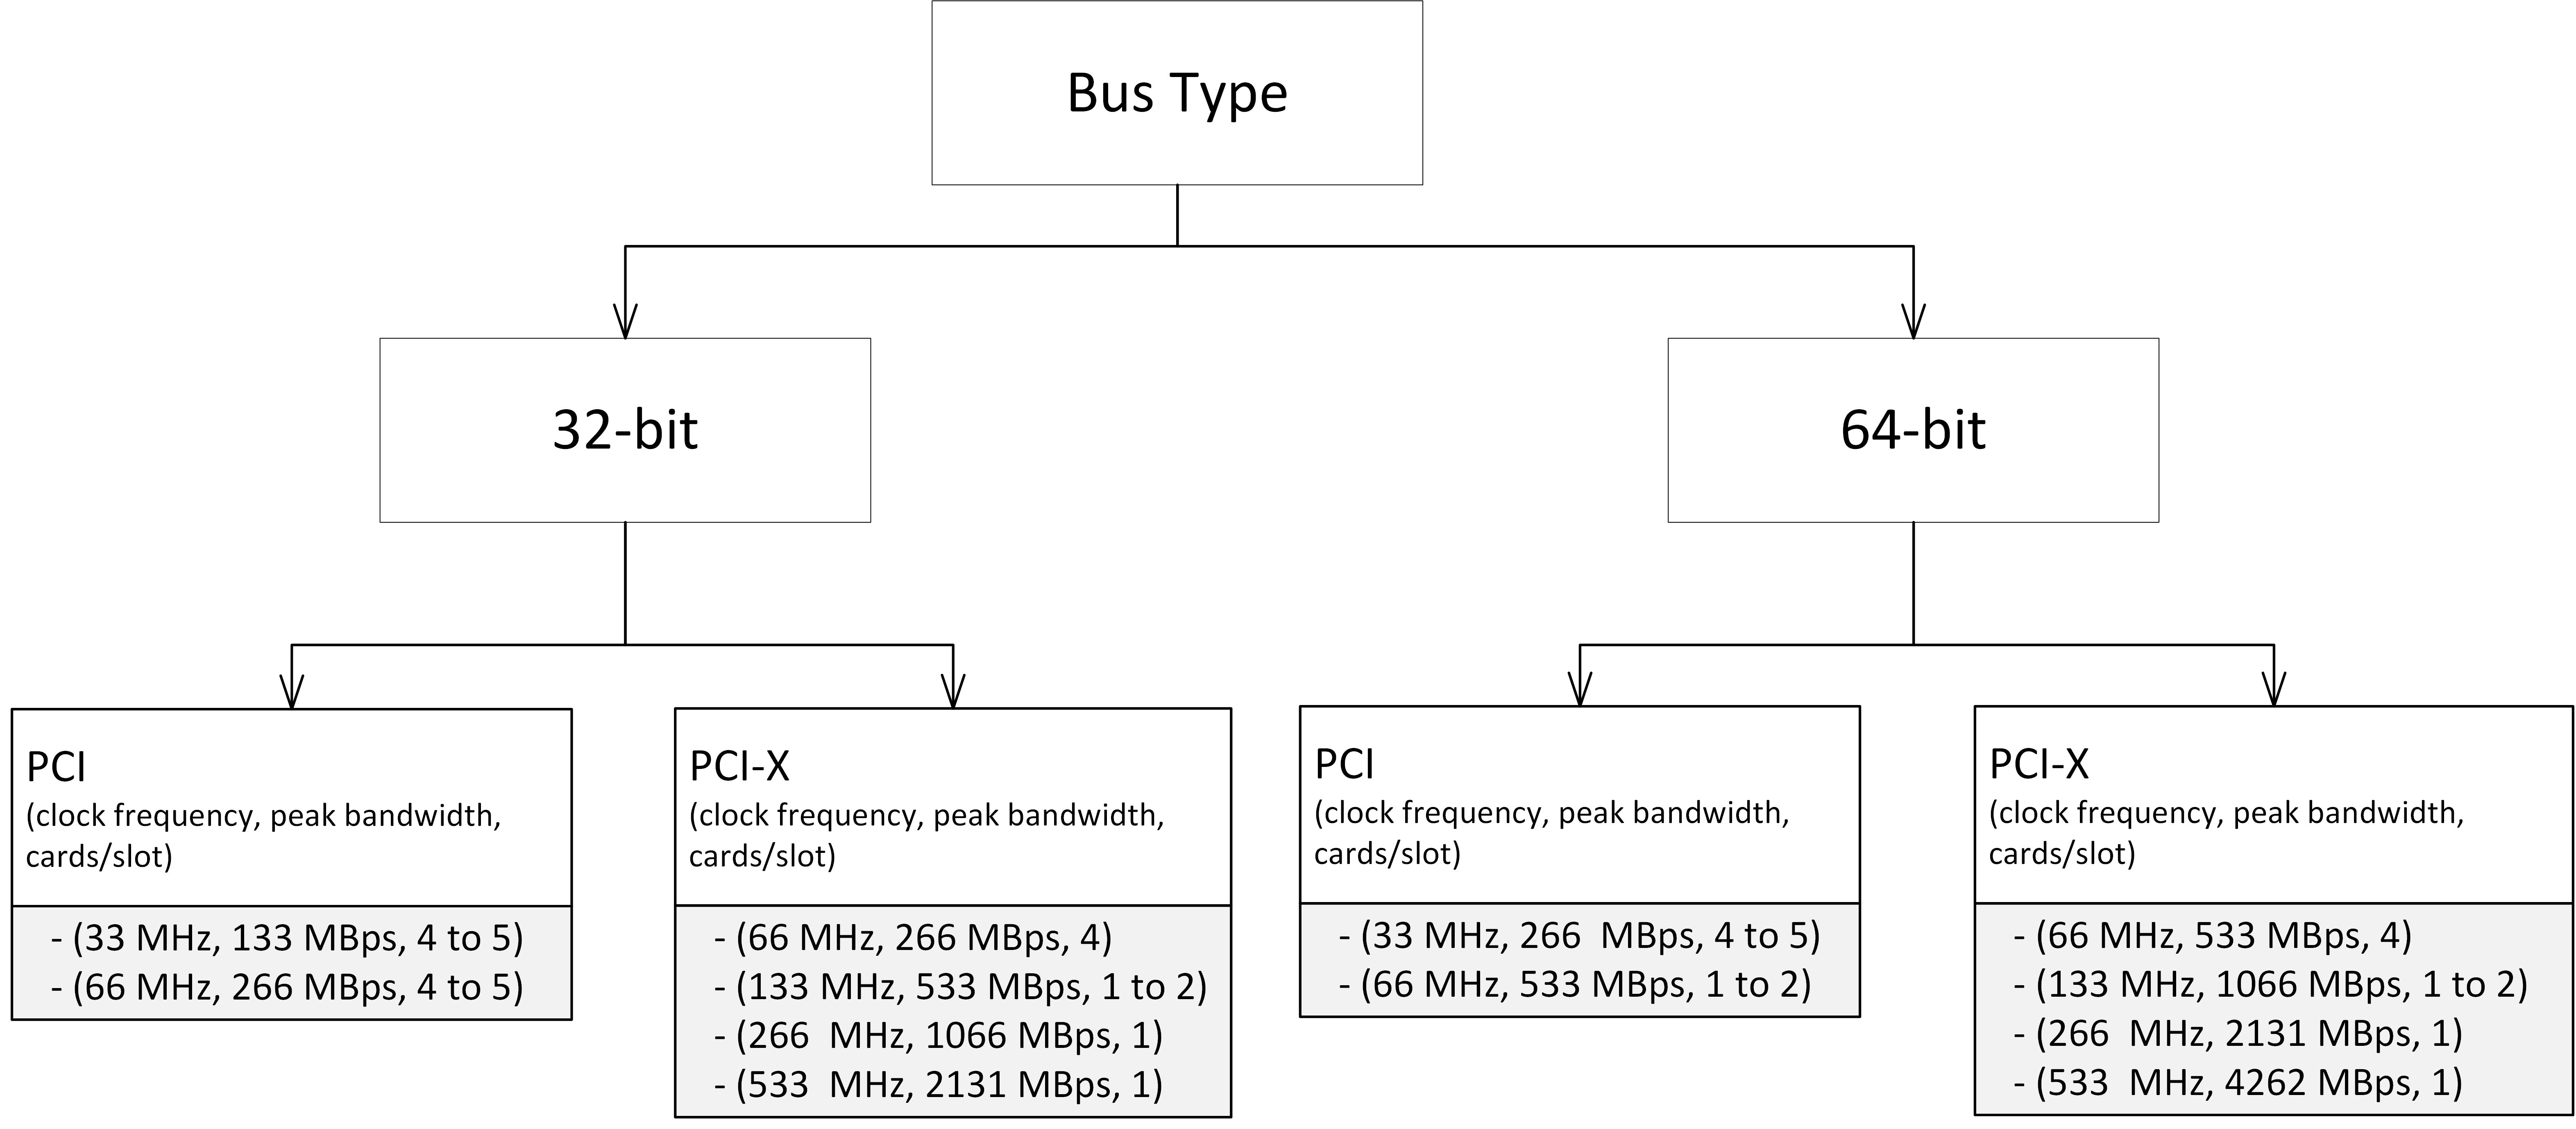
\includegraphics[width=\linewidth]{introduction/comparison-of-bus-frequency-bandwidth-slots}
	\caption{Comparison of Bus Frequency, Bandwidth and Number of Slots}\label{fig:comparison-of-bus-frequency-bandwidth-slots}
\end{figure}

A PCI express (PCIe) Interconnect that connects two devices is referred to as a Link. A link consists if either x1, x2, x4, x8, x12, x16 or x32 signal pairs in each direction. These signals are referred to as Lanes. A designer determines how many Lanes to implement based on the targeted performance benchmark required on a given Link.


The Figure \ref{fig:comparison-of-bus-frequency-bandwidth-slots} shows aggregate bandwidth numbers for various Link width implementations, as is apparent from this table, the peak bandwidth achievable with \gls{pcie} is significantly higher than any existing bus today.


